				
%% bare_conf.tex
%% V1.4a
%% 2014/09/17
%% by Michael Shell
%% See:
%% http://www.michaelshell.org/
%% for current contact information.
%%
%% This is a skeleton file demonstrating the use of IEEEtran.cls
%% (requires IEEEtran.cls version 1.8a or later) with an IEEE
%% conference paper.
%%
%% Support sites:
%% http://www.michaelshell.org/tex/ieeetran/
%% http://www.ctan.org/tex-archive/macros/latex/contrib/IEEEtran/
%% and
%% http://www.ieee.org/

%%*************************************************************************
%% Legal Notice:
%% This code is offered as-is without any warranty either expressed or
%% implied; without even the implied warranty of MERCHANTABILITY or
%% FITNESS FOR A PARTICULAR PURPOSE! 
%% User assumes all risk.
%% In no event shall IEEE or any contributor to this code be liable for
%% any damages or losses, including, but not limited to, incidental,
%% consequential, or any other damages, resulting from the use or misuse
%% of any information contained here.
%%
%% All comments are the opinions of their respective authors and are not
%% necessarily endorsed by the IEEE.
%%
%% This work is distributed under the LaTeX Project Public License (LPPL)
%% ( http://www.latex-project.org/ ) version 1.3, and may be freely used,
%% distributed and modified. A copy of the LPPL, version 1.3, is included
%% in the base LaTeX documentation of all distributions of LaTeX released
%% 2003/12/01 or later.
%% Retain all contribution notices and credits.
%% ** Modified files should be clearly indicated as such, including  **
%% ** renaming them and changing author support contact information. **
%%
%% File list of work: IEEEtran.cls, IEEEtran_HOWTO.pdf, bare_adv.tex,
%%                    bare_conf.tex, bare_jrnl.tex, bare_conf_compsoc.tex,
%%                    bare_jrnl_compsoc.tex, bare_jrnl_transmag.tex
%%*************************************************************************


% *** Authors should verify (and, if needed, correct) their LaTeX system  ***
% *** with the testflow diagnostic prior to trusting their LaTeX platform ***
% *** with production work. IEEE's font choices and paper sizes can       ***
% *** trigger bugs that do not appear when using other class files.       ***                          ***
% The testflow support page is at:
% http://www.michaelshell.org/tex/testflow/


\documentclass[12pt,journal,draftclsnofoot,onecolumn]{IEEEtran}
%\documentclass[journal]{IEEEtran}
% Some Computer Society conferences also require the compsoc mode option,
% but others use the standard conference format.
%
% If IEEEtran.cls has not been installed into the LaTeX system files,
% manually specify the path to it like:
% \documentclass[conference]{../sty/IEEEtran}





% Some very useful LaTeX packages include:
% (uncomment the ones you want to load)


% *** MISC UTILITY PACKAGES ***
%
%\usepackage{ifpdf}
% Heiko Oberdiek's ifpdf.sty is very useful if you need conditional
% compilation based on whether the output is pdf or dvi.
% usage:
% \ifpdf
%   % pdf code
% \else
%   % dvi code
% \fi
% The latest version of ifpdf.sty can be obtained from:
% http://www.ctan.org/tex-archive/macros/latex/contrib/oberdiek/
% Also, note that IEEEtran.cls V1.7 and later provides a builtin
% \ifCLASSINFOpdf conditional that works the same way.
% When switching from latex to pdflatex and vice-versa, the compiler may
% have to be run twice to clear warning/error messages.






% *** CITATION PACKAGES ***
%
%\usepackage{cite}
% cite.sty was written by Donald Arseneau
% V1.6 and later of IEEEtran pre-defines the format of the cite.sty package
% \cite{} output to follow that of IEEE. Loading the cite package will
% result in citation numbers being automatically sorted and properly
% "compressed/ranged". e.g., [1], [9], [2], [7], [5], [6] without using
% cite.sty will become [1], [2], [5]--[7], [9] using cite.sty. cite.sty's
% \cite will automatically add leading space, if needed. Use cite.sty's
% noadjust option (cite.sty V3.8 and later) if you want to turn this off
% such as if a citation ever needs to be enclosed in parenthesis.
% cite.sty is already installed on most LaTeX systems. Be sure and use
% version 5.0 (2009-03-20) and later if using hyperref.sty.
% The latest version can be obtained at:
% http://www.ctan.org/tex-archive/macros/latex/contrib/cite/
% The documentation is contained in the cite.sty file itself.






% *** GRAPHICS RELATED PACKAGES ***
%
\ifCLASSINFOpdf
  % \usepackage[pdftex]{graphicx}
  % declare the path(s) where your graphic files are
  % \graphicspath{{../pdf/}{../jpeg/}}
  % and their extensions so you won't have to specify these with
  % every instance of \includegraphics
  % \DeclareGraphicsExtensions{.pdf,.jpeg,.png}
\else
  % or other class option (dvipsone, dvipdf, if not using dvips). graphicx
  % will default to the driver specified in the system graphics.cfg if no
  % driver is specified.
  % \usepackage[dvips]{graphicx}
  % declare the path(s) where your graphic files are
  % \graphicspath{{../eps/}}
  % and their extensions so you won't have to specify these with
  % every instance of \includegraphics
  % \DeclareGraphicsExtensions{.eps}
\fi
% graphicx was written by David Carlisle and Sebastian Rahtz. It is
% required if you want graphics, photos, etc. graphicx.sty is already
% installed on most LaTeX systems. The latest version and documentation
% can be obtained at: 
% http://www.ctan.org/tex-archive/macros/latex/required/graphics/
% Another good source of documentation is "Using Imported Graphics in
% LaTeX2e" by Keith Reckdahl which can be found at:
% http://www.ctan.org/tex-archive/info/epslatex/
%
% latex, and pdflatex in dvi mode, support graphics in encapsulated
% postscript (.eps) format. pdflatex in pdf mode supports graphics
% in .pdf, .jpeg, .png and .mps (metapost) formats. Users should ensure
% that all non-photo figures use a vector format (.eps, .pdf, .mps) and
% not a bitmapped formats (.jpeg, .png). IEEE frowns on bitmapped formats
% which can result in "jaggedy"/blurry rendering of lines and letters as
% well as large increases in file sizes.
%
% You can find documentation about the pdfTeX application at:
% http://www.tug.org/applications/pdftex





% *** MATH PACKAGES ***
%
%\usepackage[cmex10]{amsmath}
% A popular package from the American Mathematical Society that provides
% many useful and powerful commands for dealing with mathematics. If using
% it, be sure to load this package with the cmex10 option to ensure that
% only type 1 fonts will utilized at all point sizes. Without this option,
% it is possible that some math symbols, particularly those within
% footnotes, will be rendered in bitmap form which will result in a
% document that can not be IEEE Xplore compliant!
%
% Also, note that the amsmath package sets \interdisplaylinepenalty to 10000
% thus preventing page breaks from occurring within multiline equations. Use:
%\interdisplaylinepenalty=2500
% after loading amsmath to restore such page breaks as IEEEtran.cls normally
% does. amsmath.sty is already installed on most LaTeX systems. The latest
% version and documentation can be obtained at:
% http://www.ctan.org/tex-archive/macros/latex/required/amslatex/math/





% *** SPECIALIZED LIST PACKAGES ***
%
%\usepackage{algorithmic}
% algorithmic.sty was written by Peter Williams and Rogerio Brito.
% This package provides an algorithmic environment fo describing algorithms.
% You can use the algorithmic environment in-text or within a figure
% environment to provide for a floating algorithm. Do NOT use the algorithm
% floating environment provided by algorithm.sty (by the same authors) or
% algorithm2e.sty (by Christophe Fiorio) as IEEE does not use dedicated
% algorithm float types and packages that provide these will not provide
% correct IEEE style captions. The latest version and documentation of
% algorithmic.sty can be obtained at:
% http://www.ctan.org/tex-archive/macros/latex/contrib/algorithms/
% There is also a support site at:
% http://algorithms.berlios.de/index.html
% Also of interest may be the (relatively newer and more customizable)
% algorithmicx.sty package by Szasz Janos:
% http://www.ctan.org/tex-archive/macros/latex/contrib/algorithmicx/




% *** ALIGNMENT PACKAGES ***
%
%\usepackage{array}
% Frank Mittelbach's and David Carlisle's array.sty patches and improves
% the standard LaTeX2e array and tabular environments to provide better
% appearance and additional user controls. As the default LaTeX2e table
% generation code is lacking to the point of almost being broken with
% respect to the quality of the end results, all users are strongly
% advised to use an enhanced (at the very least that provided by array.sty)
% set of table tools. array.sty is already installed on most systems. The
% latest version and documentation can be obtained at:
% http://www.ctan.org/tex-archive/macros/latex/required/tools/


% IEEEtran contains the IEEEeqnarray family of commands that can be used to
% generate multiline equations as well as matrices, tables, etc., of high
% quality.




% *** SUBFIGURE PACKAGES ***
%\ifCLASSOPTIONcompsoc
%  \usepackage[caption=false,font=normalsize,labelfont=sf,textfont=sf]{subfig}
%\else
%  \usepackage[caption=false,font=footnotesize]{subfig}
%\fi
% subfig.sty, written by Steven Douglas Cochran, is the modern replacement
% for subfigure.sty, the latter of which is no longer maintained and is
% incompatible with some LaTeX packages including fixltx2e. However,
% subfig.sty requires and automatically loads Axel Sommerfeldt's caption.sty
% which will override IEEEtran.cls' handling of captions and this will result
% in non-IEEE style figure/table captions. To prevent this problem, be sure
% and invoke subfig.sty's "caption=false" package option (available since
% subfig.sty version 1.3, 2005/06/28) as this is will preserve IEEEtran.cls
% handling of captions.
% Note that the Computer Society format requires a larger sans serif font
% than the serif footnote size font used in traditional IEEE formatting
% and thus the need to invoke different subfig.sty package options depending
% on whether compsoc mode has been enabled.
%
% The latest version and documentation of subfig.sty can be obtained at:
% http://www.ctan.org/tex-archive/macros/latex/contrib/subfig/




% *** FLOAT PACKAGES ***
%
%\usepackage{fixltx2e}
% fixltx2e, the successor to the earlier fix2col.sty, was written by
% Frank Mittelbach and David Carlisle. This package corrects a few problems
% in the LaTeX2e kernel, the most notable of which is that in current
% LaTeX2e releases, the ordering of single and double column floats is not
% guaranteed to be preserved. Thus, an unpatched LaTeX2e can allow a
% single column figure to be placed prior to an earlier double column
% figure. The latest version and documentation can be found at:
% http://www.ctan.org/tex-archive/macros/latex/base/


%\usepackage{stfloats}
% stfloats.sty was written by Sigitas Tolusis. This package gives LaTeX2e
% the ability to do double column floats at the bottom of the page as well
% as the top. (e.g., "\begin{figure*}[!b]" is not normally possible in
% LaTeX2e). It also provides a command:
%\fnbelowfloat
% to enable the placement of footnotes below bottom floats (the standard
% LaTeX2e kernel puts them above bottom floats). This is an invasive package
% which rewrites many portions of the LaTeX2e float routines. It may not work
% with other packages that modify the LaTeX2e float routines. The latest
% version and documentation can be obtained at:
% http://www.ctan.org/tex-archive/macros/latex/contrib/sttools/
% Do not use the stfloats baselinefloat ability as IEEE does not allow
% \baselineskip to stretch. Authors submitting work to the IEEE should note
% that IEEE rarely uses double column equations and that authors should try
% to avoid such use. Do not be tempted to use the cuted.sty or midfloat.sty
% packages (also by Sigitas Tolusis) as IEEE does not format its papers in
% such ways.
% Do not attempt to use stfloats with fixltx2e as they are incompatible.
% Instead, use Morten Hogholm'a dblfloatfix which combines the features
% of both fixltx2e and stfloats:
%
% \usepac_jage{dblfloatfix}
% The latest version can be found at:
% http://www.ctan.org/tex-archive/macros/latex/contrib/dblfloatfix/




% *** PDF, URL AND HYPERLINK PACKAGES ***
%
%\usepackage{url}
% url.sty was written by Donald Arseneau. It provides better support for
% handling and breaking URLs. url.sty is already installed on most LaTeX
% systems. The latest version and documentation can be obtained at:
% http://www.ctan.org/tex-archive/macros/latex/contrib/url/
% Basically, \url{my_url_here}.




% *** Do not adjust lengths that control margins, column widths, etc. ***
% *** Do not use packages that alter fonts (such as pslatex).         ***
% There should be no need to do such things with IEEEtran.cls V1.6 and later.
% (Unless specifically asked to do so by the journal or conference you plan
% to submit to, of course. )


% correct bad hyphenation here
\hyphenation{op-tical net-works semi-conduc-tor}
\usepackage{cite,times,amsmath,epsfig,algorithmic,array}
\usepackage{mdwmath}
\usepackage{mdwtab}
\usepackage{eqparbox}
%\usepackage{psfig}
\usepackage{cite}
\usepackage{graphicx}
\usepackage{amsfonts}
%\usepackage{intmacros}
\usepackage{epstopdf}
\usepackage{amsfonts}
\usepackage{amsmath}
\usepackage{amssymb}
\usepackage{amsthm}
\usepackage{algorithm}
\usepackage{algorithmic}


\begin{document}
%
% paper title
% Titles are generally capitalized except for words such as a, an, and, as,
% at, but, by, for, in, nor, of, on, or, the, to and up, which are usually
% not capitalized unless they are the first or last word of the title.
% Linebreaks \\ can be used within to get better formatting as desired.
% Do not put math or special symbols in the title.
\title{Robust Transmission Design for MISO Wiretap Channnel with Cooperative Jamming}


% author names and affiliations
% use a multiple column layout for up to three different
% affiliations
%\author{
%\IEEEauthorblockN{Yanqing Liu, Liang Dong and Robert J. Marks II}
%\IEEEauthorblockA{Department of Electrical and Computer Engineering\\
%Baylor University, Waco, Texas \\
%Email: \{yanqing\_liu, liang\_dong, robert\_marks\}@baylor.edu}
%}

\author{
\IEEEauthorblockN{Author 1}
%\IEEEauthorblockA{Department of Electrical and Computer Engineering\\
%Baylor University, Waco, Texas \\
%Email: \{yanqing\_liu, liang\_dong, robert\_marks\}@baylor.edu}
}

% conference papers do not typically use \thanks and this command
% is locked out in conference mode. If really needed, such as for
% the acknowledgment of grants, issue a \IEEEoverridecommandlockouts
% after \documentclass

% for over three affiliations, or if they all won't fit within the width
% of the page, use this alternative format:
% 
%\author{\IEEEauthorblockN{Michael Shell\IEEEauthorrefmark{1},
%Homer Simpson\IEEEauthorrefmark{2},
%James Kirk\IEEEauthorrefmark{3}, 
%Montgomery Scott\IEEEauthorrefmark{3} and
%Eldon Tyrell\IEEEauthorrefmark{4}}
%\IEEEauthorblockA{\IEEEauthorrefmark{1}School of Electrical and Computer Engineering\\
%Georgia Institute of Technology,
%Atlanta, Georgia 30332--0250\\ Email: see http://www.michaelshell.org/contact.html}
%\IEEEauthorblockA{\IEEEauthorrefmark{2}Twentieth Century Fox, Springfield, USA\\
%Email: homer@thesimpsons.com}
%\IEEEauthorblockA{\IEEEauthorrefmark{3}Starfleet Academy, San Francisco, California 96678-2391\\
%Telephone: (800) 555--1212, Fax: (888) 555--1212}
%\IEEEauthorblockA{\IEEEauthorrefmark{4}Tyrell Inc., 123 Replicant Street, Los Angeles, California 90210--4321}}




% use for special paper notices
%\IEEEspecialpapernotice{(Invited Paper)}




% make the title area
\maketitle

% As a general rule, do not put math, special symbols or citations
% in the abstract
\begin{abstract}
In this paper, we study physical layer security for the
downlink of cellular networks, where the confidential messages
transmitted to each user can be eavesdropped by other users in the cell. Fot the base station, the channels of all the users are not assumed to be identically distributed. The path loss, which is determined by the distance between the base station and the user, is considered. The achievalbe secrecy rate regularized channel inversion (RCI) precoding  is investigated using random matrix theory. An iterative algorithm is proposed to determine the regrlarization parameter of RCI precoding.
\end{abstract}

% no keywords




% For peer review papers, you can put extra information on the cover
% page as needed:
% \ifCLASSOPTIONpeerreview
% \begin{center} \bfseries EDICS Category: 3-BBND \end{center}
% \fi
%
% For peerreview papers, this IEEEtran command inserts a page break and
% creates the second title. It will be ignored for other modes.
\IEEEpeerreviewmaketitle



\section{Introduction}
Due to the multiple antennas, the base stations (BS) can send messages to multiple users simultaneously. This scenario is referred to
as multiuser multiple-input-single-output(MISO) downlink transmission. In order to suppress the intra-cell interference, channel inversion (CI) precoding can be deployed. The CI precoding technique can achieve can achieve the same asymptotic sum capacity as that of DPC, as the number of users goes to infinity \cite{yoo2006optimality}. However, the sum capacity grows linearly with the minimum of the number of antennas and users, the sum rate of channel inversion does not grow linearly with the number of users when the number of the antennas is equal to the number of users. This poor performance is due to the large spread
in the singular values of the channel matrix \cite{peel2005vector}. In order to address the problem, regularized channel inversion (RCI) is proposed. A regularization parameter is introduced in the CI precoding. The regularization parameter controls the amount of interference leaked to other users.  The optimal regularization parameter needs to be determined under different scenarios. When the number of users is equal to the number of antennas of the BS,  the optimal parameter is found by optimizing the large system approximation of signal-to-interference-plus-noise ratio (SINR)\cite{peel2005vector}. Using random matrix theory, the same optimal parameter has been derived. In \cite{razavi2016channel}, an adaptive RCI technique by deriving the regularization parameter as
a function of the variance of the CSI measurement error. Feedback   optimization
problems  that  maximize  the  users’  SINR  in  a  two-cell  multi-user down link transmission is studied assuming RCI precoding.  As
When considering confidential downlink transmission, the regularization
parameter and power allocation are optimized using large-system analysis~\cite{geraci2012secrecy}. In ~\cite{geraci2014physical,geraci2013linear,geraci2012secrecy,he2015base,geraci2013large,geraci2014secrecy}, the secrecy rates achievable by
RCI precoding in downlink multi-antenna cellular networks  is analyzed considering. Regularized phase alignment (RPA) \cite{razavi2014transmit,razavi2015adaptively} is investigated. RPA precoding can be viewed as first applying phase alignment operation to the messages, then using RCI to transmit the phase aligned signal.

 

%In these papers, the secrecy capacity of the MIMO wiretap
%channel was characterized. Taking the statistics of wireless
%fading into consideration, the secrecy outage probability was
%examined for Rayleigh fading [13, 14] and Nakagami-m fading
%[15, 16]. Furthermore, transmit beamforming in the direction
%of the receiver has been investigated as a practical means
%of providing secure transmission in the MIMO wiretap channel
%[17–19]. In [17], beamforming was proposed to minimize the
%transmit power for a prespecified signal-to-interference-plusnoise
%ratio (SINR) at the receiver. In [18], artificial noise
%was incorporated in the beamforming weights to constrain
%the maximum SINRs of the eavesdroppers. Applying linear
%precoding at the transmitter, [19] adopted a game-theoretic
%formulation to balance performance and fairness. These beamforming
%methods mandate precise channel state information
%(CSI) of the eavesdropper’s channel and/or the main channel.
%This incurs high feedback overhead and computational cost
%of signal processing, especially for large numbers of transmit
%antennas [20]. Against this background, antenna selection was
%applied at the multi-antenna transmitter to enhance security
%with reduced hardware complexity [21, 22]. In [23], the effect
%of antenna selection at the multi-antenna relay on security
%improvement was examined for amplify-and-forward relaying
%and cooperative jamming. 

In this paper, the secure donw-link transmission of multi-user MIMO system is studied. Different from the work in \cite{geraci2012secrecy,geraci2014physical}, the path loss which is determined by the distance between the base station and the user is considered. A iterative algorithm  based on the distribution of the distance is proposed to determine the regularization parameter.

\emph{Notations:} Subscripts $[\cdot]^T$T and $[\cdot]^H$ mean the transpose and
the conjugate transpose, respectively. We use $\mathbf{I}_{N}$  to denote the
$N$-dimensional identity matrix, and. $\mathbb{E}[\cdot]$ is the expection operation. $\mathbb{C}^{m \times n}$ denotes the space of all $m \times n$ matrices
with complex-valued elements. Notation $\mathbf{x} \sim \mathbb{CN}(\mathbf{0},\mathbf{\Sigma})$ reperents a
circularly symmetric complex Gaussian vector $\mathbf{x}$  with
zero mean and covariance matrix $\mathbf{\Sigma}$.

\section{System Model} \label{sec:system model}
We investigate the secure downlink data transmission of a narrow band multi-user MIMO system, as depicted in \ref{fig:system}. The narrowband channels
between the BS and the users is assumed. In the system, the BS equipped with $N$ antennas sends confidential messages to $K$ users simultaneously. 
For each user, the other $K - 1$ users are malicious users. 
We assume that the
channels are time-invariant with the transmission time-scale
under consideration. 
\begin{figure}[!htbp]
	\centering
	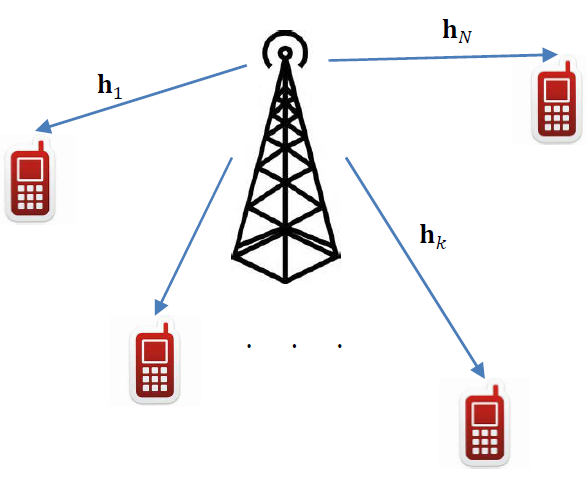
\includegraphics[width=8.7cm]{system.png} % requires the graphicx package
	\caption{Illustration of a downlink data transmission of a cellular network.}
	\label{fig:system}
\end{figure}

The received signal of the $k$th user is 
\begin{eqnarray}
y_k = P \mathbf{h}_{k}\mathbf{w}_{k}s_k +P \sum_{j \neq k}\mathbf{h}_k\mathbf{w}_js_j + n_k
\end{eqnarray}
where $\mathbf{h}_i \in \mathbb{C}^{1 \times N}$ is the channel from the BS to the $k$th user; $\mathbf{w}_i \in \mathbb{C}^{N \times 1}$ is the beamforming vector of the $k$th user. $P$ is the transmission power. Assume that the $s_i$ and $s_j$ are independent and $E[s_i] = 1$. Let the combined channel $\mathbf{H} = [\mathbf{h}_1^T,\cdots,\mathbf{h}_K^T]^T$, and combined precoding matrix $\mathbf{W} = [\mathbf{w}_1,\cdots,\mathbf{w}_K]$. The received signal of the $K$ user can be rewritten as
\begin{eqnarray}
\mathbf{y} = P\mathbf{H}\mathbf{W}\mathbf{s} + \mathbf{n}
\end{eqnarray}
where $\mathbf{s} = [s_1,\cdots,s_k]^T$, $\mathbf{y} = [y_1,\cdots,y_k]^T$ and $\mathbf{n} = [n_1,\cdots,n_k]^T$. We imopose the power constraint $\mathrm{Tr}\left(\mathbf{W}\mathbf{W}^H\right)=1$. Ande denote $\beta = N/K$. We also define thenominal SNR as $\rho = P/\sigma^2 = K/\sigma^2$.

\section{Generalized Regularized Channel Inversion and some old}
In this paper, we propose Generalied regularized channle inversin (GRCI). For comparison, some old results are presented first.
\subsection{RCI}
It is shown that channel inversion (CI) precoder has worse performance than the RCI precoder when SNR is low, although CI can cancel all the all the interference caused by other users. The prcoding matrix is
\begin{eqnarray}
	\mathbf{W} &=& \frac{1}{\sqrt{\zeta_R}}\mathbf{H}^H\left(\mathbf{H}\mathbf{H}^H + \alpha\mathbf{I}\right)^{-1}
	%&=&\frac{1}{\sqrt{\zeta}}\left(\mathbf{H}^H\mathbf{H} + \Lambda \mathbf{I}\right)^{-1}\mathbf{H}^H
\end{eqnarray}
where
\begin{equation} \label{eq:zeta_R}
	\zeta_R = \mathrm{Tr}\left(\mathbf{H}\mathbf{H}^H\left(\mathbf{H}\mathbf{H}^H + \alpha\mathbf{I}\right)^{-2}\right)
\end{equation}
is used to guarantee the transmit power constrant $\mathrm{Tr}\left(\mathbf{W}\mathbf{W}^H\right) = 1$. The choice of regularization paremeter is well-known $\alpha = \frac{1}{\beta\rho}$

\subsection{Downlink transmit beamforming with quality of service (QoS) constraints}
The problem of guaranteeding the QoS of each user is 
\begin{equation}
\begin{aligned} \label{eq:problem_qos}
& \underset{\mathbf{x},\gamma}{\text{maximize}}
& & \gamma \\
& \text{subject to}
& &  \frac{P|\mathbf{h}_{k}\mathbf{w}_k|^2}{P\sum_{j \neq k}|\mathbf{h}_{k}\mathbf{w}_j|^2 + \sigma^2} \geq \gamma\\
&&& \sum_{k = 1}^{K}\|\mathbf{w}_k\|^2 \leq 1.
\end{aligned}
\end{equation}
The problem can be solved as a series of SOCP feasibility problems using bisection search.



The eigen decomposition of $\mathbf{H}\mathbf{H}^H$ is
\begin{equation}
	\mathbf{H}\mathbf{H}^H = \mathbf{U}\mathbf{\Lambda}\mathbf{U}^H
\end{equation}

 

\begin{eqnarray}
\mathbf{W} &=& \frac{1}{\sqrt{\zeta}}\mathbf{H}^H\left(\mathbf{H}\mathbf{H}^H + \mathbf{U}\mathbf{\Xi}\mathbf{U}^H\right)^{-1}
%&=&\frac{1}{\sqrt{\zeta}}\left(\mathbf{H}^H\mathbf{H} + \Lambda \mathbf{I}\right)^{-1}\mathbf{H}^H
\end{eqnarray}
where $\mathbf{\Xi} = \mathrm{diag}(\xi_1,\cdots,\xi_K)$
\begin{equation} \label{eq:zeta}
\zeta = \mathrm{Tr}\left(\mathbf{H}\mathbf{H}^H\left(\mathbf{H}\mathbf{H}^H + \mathbf{U}\mathbf{\Xi}\mathbf{U}^H\right)^{-2}\right)
\end{equation}
is used to guarantee the transmit power constrant $\mathrm{Tr}\left(\mathbf{W}\mathbf{W}^H\right) = 1$. The eigen decomposition of $\mathbf{H}\mathbf{H}^H$ is
\begin{equation}
\mathbf{H}\mathbf{H}^H = \mathbf{U}\mathbf{\Lambda}\mathbf{U}^H
\end{equation}
%The SVD of $\mathbf{H}$ is
%\begin{eqnarray}
%\mathbf{H} = \mathbf{U}\mathbf{\Lambda}^{1/2}\mathbf{V}^H
%\end{eqnarray}
We obtain
\begin{eqnarray} \label{eq:zeta_futher}
\zeta &=& \mathrm{Tr}\left(\mathbf{U}\mathbf{\Lambda}^2\mathbf{U}^H\left(\mathbf{U}\left(\mathbf{\Lambda} + \mathbf{\Xi}\right)\mathbf{U}^H\right)^{-2}\right)\\
&=& \mathrm{Tr}\left(\mathbf{\mathbf{\Lambda}\left(\mathbf{\Lambda} + \mathbf{\Xi}\right)^{-2}}\right). \label{eq:zeta_docompose}
\end{eqnarray}

The received signal of the $k$th user is then
\begin{eqnarray}
y_k 
&=&\frac{1}{\sqrt{\zeta}}\mathbf{h}_k\mathbf{H}^H\left(\mathbf{H}\mathbf{H}^H + \mathbf{U}\mathbf{\Xi}\mathbf{U}^H\right)^{-1}\mathbf{e}_{k}s_k \nonumber \\ 
&&+\frac{1}{\sqrt{\zeta}}\sum_{j \neq k}\mathbf{h}_k\mathbf{H}^H\left(\mathbf{H}\mathbf{H}^H + \mathbf{U}\mathbf{\Xi}\mathbf{U}^{H}\right)^{-1}\mathbf{e}_js_j + n_k\\
 &=&\frac{1}{\sqrt{\zeta}}\mathbf{h}_k\mathbf{H}^H\mathbf{U}\left(\mathbf{\Lambda} + \mathbf{\Xi}\right)^{-1}\mathbf{U}_{k*}^Hs_k \nonumber\\
&&+ \frac{1}{\sqrt{\zeta}}\sum_{j \neq k}\mathbf{h}_k\mathbf{H}^H\mathbf{U}\left(\mathbf{\Lambda} + \mathbf{U}\mathbf{\Xi}\mathbf{U}^H\right)^{-1}\mathbf{U}_{j*}^Hs_j + n_k
\end{eqnarray}
%The received signal of the potential eavesdroppers is 
%\begin{eqnarray}
%\mathbf{y}_k &=& \frac{1}{\sqrt{\zeta}}\mathbf{H}_k\mathbf{H}^H\left(\mathbf{H}\mathbf{H}^H + \mathbf{U}\mathbf{\Xi}\mathbf{U}^H\right)^{-1}\mathbf{e}_ks_k + \mathbf{m}\\
%&=&\frac{1}{\sqrt{\zeta}}\mathbf{H}_k\mathbf{H}^H\mathbf{U}\left(\mathbf{\Lambda} + \mathbf{\Xi}\right)^{-1}\mathbf{U}_{k*}^Hs_k + \mathbf{m} \label{eq:received_eavesdropper}
%\end{eqnarray}
%where $\mathbf{y}_k$ is the vector $\mathbf{y}$ with the $k$th element removed; $\mathbf{H}_k$ is matrix $\mathbf{H}$ with the $k$th row removed; $\mathbf{m} \sim \mathbb{C}\mathbb{N}(\mathbf{0},\mathbf{I}_{K-1})$.
%In \eqref{eq:received_eavesdropper}, it is assumed $K-1$ eavesdroppers can cooperate and perform interference cancellation, and undesired signal term apart from the received noise $\mathbf{m}$ is cancelled \cite{geraci2012secrecy}.
%
%The received signal of the $k$th user is 
where $\mathbf{x} = [x_1,\cdots,x_K]^T$ and $x_k = 1/(\lambda_k + \xi_k)$. $\mathbf{a}_{kj}^H = \mathbf{h}_k\mathbf{V}\mathbf{\Lambda}^{1/2}\mathrm{diag}(\mathbf{U}_{j*}^H)$.
The SINR of the $k$th user is
\begin{eqnarray}
\gamma_k &=& \frac{ |\mathbf{h}_k\mathbf{H}^H\mathbf{U}\left(\mathbf{\Lambda} + \mathbf{\Xi}\right)^{-1}\mathbf{U}_{k*}^H|^2}{\sum_{j \neq k}|\mathbf{h}_k\mathbf{H}^H\mathbf{U}\left(\mathbf{\Lambda} + \mathbf{\Xi}\right)^{-1}\mathbf{U}_{j*}^H|^2 + \zeta\sigma^2}\\
&=&\frac{|t_k|^2}{t_{\tilde{k}}^2 + \zeta \sigma^2}
\end{eqnarray}
where
\begin{eqnarray}
	t_k &=& \mathbf{h}_k\mathbf{H}^H\mathbf{U}\left(\mathbf{\Lambda} + \mathbf{\Xi}\right)^{-1}\mathbf{U}_{k*}^H\\
	& = &\mathbf{h}_k\mathbf{H}^H\mathbf{U}\mathrm{diag}(\mathbf{U}_{k*}^H)\mathbf{x}\\
%	&=& \mathbf{h}_k\mathbf{V}\mathbf{\Lambda}^{1/2}\mathrm{diag}(\mathbf{U}_{k*}^H)\mathbf{x} \label{eq:diag_times_vector}\\
	&=& \mathbf{a}_{kk}^H\mathbf{x}. \label{eq:SINR_k}
\end{eqnarray}
%Equation \ref{eq:diag_times_vector} from the fact that $\mathrm{diag}(\mathbf{x})\mathbf{y} = \mathrm{diag}(\mathbf{y})\mathbf{x}$. (Have been tested by Matlab)

%\begin{eqnarray}
%t_k &=& \mathrm{Tr}\left(\mathbf{U}_{k*}^H\mathbf{h}_k\mathbf{H}^H\mathbf{U}\left(\mathbf{\Lambda} + \mathbf{\Xi}\right)^{-1}\right)\\
%& = &\sum_{i = 1}^{K}\mathbf{A}_{k,ii}/(\lambda_i + \xi_i)
%\end{eqnarray}
\begin{eqnarray}
t_{\tilde{k}}^2 &=& \sum_{j \neq k}|\mathbf{h}_k\mathbf{H}^H\mathbf{U}\left(\mathbf{\Lambda} + \mathbf{\Xi}\right)^{-1}\mathbf{U}_{j*}^H|^2\\
&=&\sum_{j \neq k}|\mathbf{a}_{kj}^H\mathbf{x}|^2
\end{eqnarray}
According to equation \eqref{eq:zeta_docompose}, we obtain
\begin{eqnarray}
\zeta &=& \mathbf{x}^T\mathbf{\Lambda}\mathbf{x}
\end{eqnarray}
%where $\mathbf{b} = [\sqrt{\lambda_1},\cdots,\sqrt{\lambda_K}]^T$.
From \eqref{eq:SINR_k}, the SINR of the $k$th user is
\begin{eqnarray}
\gamma_k &=& \frac{|\mathbf{a}_{kk}^H\mathbf{x}_k|^2}{\sum_{j \neq k}|\mathbf{a}_{kj}^H\mathbf{x}|^2 + \sigma^2\mathbf{x}^T\mathbf{\Lambda}^T\mathbf{x}}\\
&=&  \frac{|\mathbf{a}_{kk}^H\mathbf{x}_k|^2}{\mathbf{x}^H\left(\mathbf{A}_{\tilde{k}} + \sigma^2\mathbf{\Lambda}\right)\mathbf{x}}.
\end{eqnarray}
where $\mathbf{A}_{\tilde{k}} = \sum_{j \neq k}\mathbf{a}_{kj}\mathbf{a}_{kj}^H$.


%\subsection{Maximize Sum-rate}
%The optimization problem is
%\begin{equation}
%\begin{aligned} \label{eq:problem2}
%& \underset{\mathbf{x}}{\text{maximize}}
%& & \sum_{i = 1}^{N}\mathrm{log}(1 + \frac{\mathbf{x}^H\mathbf{A}_k\mathbf{x}}{\mathbf{x}^H \left(\mathbf{A}_{\tilde{k}} + \mathbf{B}\right)\mathbf{x}}) \\
%& \text{subject to}
%& &  \mathbf{e}_i^T\mathbf{x}\mathbf{x}^T\mathbf{e}_i \leq \lambda_i^{-2}, i=1, \cdots, K.
%\end{aligned}
%\end{equation}
%
%
%\subsection{Qos}
%The optimization problem is
%\begin{equation}
%\begin{aligned} \label{eq:problem2}
%& \underset{\mathbf{x},t}{\text{maximize}}
%& & t \\
%& \text{subject to}
%& &  \frac{\mathbf{x}^H\mathbf{A}_k\mathbf{x}}{\mathbf{x}^H \left(\mathbf{A}_{\tilde{k}} + \mathbf{B}\right)\mathbf{x}} \geq t\\
%&&&\mathbf{e}_i^T\mathbf{x}\mathbf{x}^T\mathbf{e}_i \leq \lambda_i^{-2}, i=1, \cdots, K.
%\end{aligned}
%\end{equation}


\emph{Proposition 1:} The elements of the vector $\mathbf{a}_{kk}$ are postive.

\emph{Proof:} Quantitie $ t_k s_k$ is the unnormalized desired signal of $k$th users. We have 
\begin{eqnarray}
\mathbf{H}\mathbf{s} &=& \mathbf{H}\mathbf{H}^H\left(\mathbf{H}\mathbf{H}^H + \mathbf{U}\mathbf{\Xi}\mathbf{U}^H\right)^{-1}\\
&=&\mathbf{U}\mathrm{diag}(\mathbf{\Lambda}(\mathbf{\Lambda} + \mathbf{\Xi}))^{-1}\mathbf{U}^H \label{eq:Hs}
\end{eqnarray}
The unnormalized signal and interference received by the $k$th user is the
$k$th entry of $\mathbf{H}\mathbf{s}$. We can obtain this	 entry
\begin{eqnarray}
[\mathbf{H}\mathbf{s}]_k = \left[u_{k,1}\frac{\lambda_1}{\lambda_1 + \xi_1}, \cdots, u_{k,K}\frac{\lambda_K}{\lambda_K + \xi_K}\right] \times 
\begin{bmatrix}
u_{1,1}^*  & \cdots & u_{K,1}^* \\
\vdots   & \ddots & \vdots  \\
u_{1,K}^*  & \cdots & u_{K,K}^* 
\end{bmatrix} \times 
\begin{bmatrix}
s_{1}\\
\vdots\\
s_{K} 
\end{bmatrix}
\end{eqnarray} \label{eq:signal_interference_k}
where $u_{k,j}$ is the $(k,j)$th entry of the matrix $\mathbf{U}$. Then the unnormalized desired signal in \eqref{eq:signal_interference_k} is
\begin{equation}
\sum_{j = 1}^{K}\left(\frac{\lambda_j}{\lambda_j + \xi_j}|u_{k,j}|^2\right) = t_k*s_k = \mathbf{a}_{kk}^H\mathbf{x}
\end{equation}
Then we obtain
\begin{equation}
\mathbf{a}_{kk} = \left[\lambda_1|u_{k,1}|^2, \cdots, \lambda_k|u_{k,K}|^2\right]^T
\end{equation}
The elements of the vector $\mathbf{a}_{kk}$ are positive. \hfill$\blacksquare$ 
\subsection{Max qos} 
The maximin SINR balancing can be cast as
\begin{equation}
\begin{aligned} \label{eq:problem_maximin}
& \underset{\mathbf{x}}{\text{maximize}}
& & \text{min} \alpha_k\gamma_k \\
& \text{subject to}
&& x_k \leq \lambda_k^{-1}, k=1, \cdots, K.
\end{aligned}
\end{equation}
Problem \eqref{eq:problem_maximin} can be equivalently reformulated as
\begin{equation}
\begin{aligned} \label{eq:problem_maximin_transformed}
& \underset{\mathbf{x},\gamma}{\text{maximize}}
& & \gamma \\
& \text{subject to}
& &  \frac{|\mathbf{a}_{kk}^H\mathbf{x}_k|^2}{\mathbf{x}^H \left(\mathbf{A}_{\tilde{k}} + \sigma^2\mathbf{\Lambda}\right)\mathbf{x}} \geq \gamma\\
&&& x_k \leq \lambda_k^{-1}, k=1, \cdots, K.
\end{aligned}
\end{equation}

Based on Proposition 1, the constraints in \eqref{eq:problem_maximin_transformed} can be transformed to second order cone (SOC) constraints for fixed $\gamma$ as
\begin{equation}
\|\left(\mathbf{A}_{\tilde{k}} + \sigma^2\mathbf{\Lambda}\right)^{1/2}\mathbf{x}\| \leq \sqrt{\frac{\alpha_k}{\gamma}}\mathbf{a}_{kk}^T\mathbf{x}
\end{equation}


\subsection{subotimal solution}
Solving problem \eqref{eq:problem_maximin_transformed} needs convex optimization tools. In order to reduce the complexity. We propose another algorithm  which can determine the regularization parameter while keeping the computational complexity low.

The total power in $\mathbf{H}\mathbf{s}$ 
\begin{eqnarray}
\|\mathbf{H}\mathbf{s}\|^2 = \sum_{k = 1}^{K}\frac{\lambda_k^2}{(\lambda_k + \xi_k)^2}
\end{eqnarray}

We find the epected power of desired signal. The expection is taken over $\mathbf{U}$. Similar to the arguments in \cite{peel2005vector}, we obtain
\begin{eqnarray}
\mathrm{Desired} &=& \mathrm{E}\left(\sum_{k = 1}^{K}\frac{\lambda_j}{\lambda_j + \xi_j}|u_{k,j}|^2\right)\\
&=&\frac{1}{K(K+1)}\left[\left(\sum_{k=1}^{K}\frac{\lambda_k}{\lambda_k + \xi_k}\right)^2 + \sum_{k = 1}^{K}\left(\frac{\lambda_k}{\lambda_k + \xi_k}\right)^2\right]	
\end{eqnarray}

The large-$K$ approximation to the SINR is
\begin{eqnarray}
\mathrm{SINR} \approx \frac{\left(\sum_{k=1}^{K}\frac{\lambda_k}{\lambda_k + \xi_k}\right)^2}{\sigma^2K^2\sum_{k=1}^{K}\frac{\lambda_k}{(\lambda_k + \xi_k)^2} +	 K\sum_{k = 1}^{K}\left(\frac{\lambda_k}{\lambda_k + \xi_k}\right)^2 - \left(\sum_{k=1}^{K}\frac{\lambda_k}{\lambda_k + \xi_k}\right)^2}
\end{eqnarray}
Let $\frac{\lambda_k}{\lambda_k + \xi_k} = y_k$, we obtain
\begin{eqnarray}
\mathrm{SINR} \approx \frac{\left(\sum_{k=1}^{K}y_k\right)^2}{\sigma^2K^2\sum_{k=1}^{K}\frac{y_k^2}{\lambda_k} +	 K\sum_{k=1}^{K}y_k^2 - \left(\sum_{k=1}^{K}y_k\right)^2}
\end{eqnarray}
We find the stationary points by setting the derivative of $\mathrm{SINR}$ to zero
\begin{eqnarray}
\frac{d}{dy_k} \frac{\left(\sum_{k=1}^{K}y_k\right)^2}{\sigma^2K^2\sum_{k=1}^{K}\frac{y_k^2}{\lambda_k} +	 K\sum_{k=1}^{K}y_k^2 - \left(\sum_{k=1}^{K}y_k\right)^2} = 0
\end{eqnarray}
After the algebraic manipulations, we obtain
\begin{eqnarray}
&&\left(\sum_{k=1}^{K}y_k\right)\left(\sigma^2K^2\sum_{k=1}^{K}\frac{y_k^2}{\lambda_k} +	 K\sum_{k=1}^{K}y_k^2 - \left(\sum_{k=1}^{K}y_k\right)^2\right) \\
&-& \left(\sum_{k=1}^{K}y_k\right)^2\left(\sigma^2K^2\frac{y_k}{\lambda_k} + Ky_k - \sum_{k=1}^{K}y_k\right)\\
&=&\sigma^2K^2\sum_{k=1}^{K}y_k\sum_{k=1}^{K}\frac{y_k^2}{\lambda_k} + K\sum_{k=1}^{K}y_k\sum_{k=1}^{K}y_k^2- \left(\sum_{k=1}^{K}y_k\right)^3\\
&& - \sigma^2K^2\left(\sum_{k=1}^{K}y_k\right)^2\frac{y_k}{\lambda_k} - K\left(\sum_{k=1}^{K}y_k\right)^2y_k + \left(\sum_{k=1}^{K}y_k\right)^3 = 0
\end{eqnarray}
Then we obtain
\begin{eqnarray}
\sigma^2K\sum_{i \neq k}\frac{y_i^2}{\lambda_i} + \sum_{i\neq k}y_i^2 = \sigma^2K\left(\sum_{i\neq k}y_i\right)\frac{y_k}{\lambda_k} +\left( \sum_{i\neq k}y_i\right)y_k
\end{eqnarray}
\begin{eqnarray}
y_k = \frac{\sigma^2K\sum_{i \neq k}\frac{y_i^2}{\lambda_i} + \sum_{i\neq k}y_i^2}{\sigma^2K\sum_{i \neq k}\frac{y_i}{\lambda_k} + \sum_{i\neq k}y_i}
\end{eqnarray}

%Let $\mathbf{y}=\left(\mathbf{A}_{\tilde{k}} + \sigma^2\mathbf{I}\right)^{1/2}\mathbf{x}$.
%Then
%\begin{eqnarray}
%	&&\mathbf{x}=\left(\mathbf{A}_{\tilde{k}} + \sigma^2\mathbf{I}\right)^{-1/2}\mathbf{y}\\
%	&&\mathbf{e}_i^T\mathbf{x}\mathbf{x}^T\mathbf{e}_i \\
%	&=&\mathbf{e}_i^T\left(\left(\mathbf{A}_{\tilde{k}} + \sigma^2\mathbf{I}\right)^{-1/2}\mathbf{y}\mathbf{y}^H\left(\mathbf{A}_{\tilde{k}} + \sigma^2\mathbf{I}\right)^{-1/2}\right)\mathbf{e}_i\\
%	&=& \mathbf{y}^H\left(\mathbf{A}_{\tilde{k}} + \sigma^2\mathbf{I}\right)^{-1/2}\mathbf{I}_k\left(\mathbf{A}_{\tilde{k}} + \sigma^2\mathbf{I}\right)^{-1/2}\mathbf{y}
%\end{eqnarray}
%
%
%We relax the constaint $\mathrm{rank}(\mathbf{Q}) = 1$,
%the optimization problem is
%\begin{equation}
%\begin{aligned} \label{eq:problem2}
%& \underset{\mathbf{x},t}{\text{maximize}}
%& & t \\
%& \text{subject to}
%& &  \frac{\mathrm{Tr}\left(\mathbf{A}_k\mathbf{Q}\right)}{\mathrm{Tr}\left(\left(\mathbf{A}_{\tilde{k}} + \sigma^2\mathbf{\Lambda}\right)\mathbf{Q}\right)} \geq t\\
%&&&\mathrm{Tr}\left(\mathbf{I}_k^T\mathbf{Q}\right) \leq \lambda_i^{-2}, k=1, \cdots, K.
%\end{aligned}
%\end{equation}









%
%
%\begin{algorithm}
%	\caption{}\label{alg:regularization parameter}
%	\begin{algorithmic}
%		\item[0.] Set initial value $m(-\rho)$$\tau_{\mathrm{min}}$ to a small value, such as $\tau_{\mathrm{min}} = \Gamma/N$. 
%		\item[1.] Solve \eqref{eq:subproblem1} for each helper with $\tau_i = \tau_{\mathrm{min}}$ to get $\mathbf{Q}_i$, and calculate the transmit efficiency $\varepsilon_i = \frac{\tau_{\mathrm{min}}}{\mathrm{Tr}(\mathbf{Q}_i)}$. If \eqref{eq:subproblem1} is infeasible, set $\varepsilon_i = 0$.
%		\item[2.] Broadcast $\varepsilon_i$ and $P_i$ to other helpers. 
%		\item[3.] For each helper set $\mathcal{E} =\{ {\varepsilon_i,\ldots, \varepsilon_N}\}$ and $\mathcal{I} =\{\}$.
%		\item[4.] For each helper find the maximum transmit efficiency in set $\mathcal{E}$, that is $\varepsilon_i = \max~\mathcal{E}$ (if $\mathcal{E}$ is empty,  the maximum transmit efficiency returned is 0). If $\varepsilon_i = 0$, goto step 6; else $\mathcal{I} := \mathcal{I} + \{i\}$; $\mathcal{E} := \mathcal{E}  - \{\varepsilon_i\}$.
%		\item[5.] If $\Gamma \geq \varepsilon_{i} P_i$, $\mathbf{Q}_{i}^* = \frac{P_i}{\mathrm{Tr(\mathrm{Q}}_i)}\mathbf{Q}_i$, $\Gamma := \Gamma - \varepsilon_iP_i$, goto step 4; else $\mathbf{Q}_{i}^* = \frac{\Gamma}{\tau_\mathrm{min}}\mathbf{Q}_i$, go to step 7.
%		\item[6.] The required secrecy rate cannot be guaranteed.
%		\item[7.] If $i \in \mathcal{I}$, the transmit covariance of Helper-$i$ is $\mathbf{Q}_i^*$, otherwise the transmit covariance is $\mathbf{0}$.
%		
%	\end{algorithmic}
%\end{algorithm}


%\section{When T = I }
%When $N \to \infty$
%\begin{eqnarray}
%\mathrm{SINR}_k = \frac{g(c,\rho)^2}{\left[1 + (1 + g(c,\rho)^2)\sigma^2\right]\left[g(c,\rho) + \rho\frac{d}{d\rho}g(c,\rho)\right]}
%\end{eqnarray}
%
%Assume there are $M$ relays each with the $N$ antennas. And there are $K$ users. The combined channels are $\mathbf{H}_m$. The received signal of $k$th MT is
%\begin{eqnarray}
%y_k = \sum_{m = 1}^{M}\mathbf{h}_{mk}\left(\mathbf{H}_m^H\mathbf{H}_m + \alpha_m\mathbf{I}\right)^{-1}\mathbf{h}_{mk}^Hs_k + \sum_{m=1}^{M}\sum_{j \neq k}\mathbf{h}_{mk}\left(\mathbf{H}_m^H\mathbf{H}_m + \alpha_m\mathbf{I}\right)^{-1}\mathbf{h}_{mj}^H s_j + n_k
%\end{eqnarray}
%
%\begin{eqnarray}
%\mathrm{SINR}_k = \frac{\sum_{m = 1}^{M}l_mg(c,\rho)}{\left[\left(\sum_{m = 1}^{M}l_m + (1 + g(c,\rho))^2\right)\right]\left[g(c,\rho) + \rho\frac{d}{d\rho}g(c,\rho)\right]}
%\end{eqnarray}
%
%
%\begin{eqnarray}
%&&\mathrm{Tr}\left(\mathbf{H}_k^H\mathbf{H}_k + \alpha\mathbf{I}\right)^{-1}\\
%&=&\frac{1}{N}\mathrm{Tr}\left(\frac{1}{N}\mathbf{H}_k^H\mathbf{H}_k + \alpha N\mathbf{I}\right)^{-1} 
%\end{eqnarray}
%
%If there is another helper. The hepler using zero forcing strategy to generate inteference to the eavesdropper. We assume that the transmit covriance of the noise is $\mathbb{N}(0, \mathbf{P_{\vert}\mathbf{I}})$
%The interference generated to the eavesdropper is
%\begin{eqnarray}
%&&\frac{1}{\sqrt{\eta}}\mathbf{f}_{\tilde{k}}\mathbf{F}_{\tilde{k}}\mathbf{P}_{\perp}\mathbf{s}\mathbf{s}\mathbf{P}_{\perp}\mathbf{F}_{\tilde{k}}\mathbf{f}_{\tilde{k}}^H\\
%&=&\frac{1}{\sqrt{\eta}}\mathbf{f}_{\tilde{k}}\mathbf{F}_{\tilde{k}}\mathbf{P}_{\perp}\mathbf{P}_{\perp}\mathbf{F}_{\tilde{k}}\mathbf{f}_{\tilde{k}}^H
%\end{eqnarray}
%where $\eta = \mathrm{tr}(\mathbf{P}_{\perp})$.
%So, when $N \to \infty$
%\begin{eqnarray}
%\mathbf{Tr}(\frac{1}{\eta}\mathbf{F}_{\tilde{k}}\mathbf{P}_{\perp}\mathbf{P}_{\perp}\mathbf{F}_{\tilde{k}}) = 1
%\end{eqnarray}
%$\mathbf{F}_{\tilde{k}}\mathbf{P}_{\perp}\mathbf{P}_{\perp}\mathbf{F}_{\tilde{k}} \sim \mathcal{W}_N(N-k, I)$, then
%\begin{eqnarray}
%&&\lim_{N \to \infty}\frac{1}{\eta}\mathbf{f}_{\tilde{k}}\mathbf{F}_{\tilde{k}}\mathbf{P}_{\perp}\mathbf{P}_{\perp}\mathbf{F}_{\tilde{k}}\mathbf{f}_{\tilde{k}}^H\\
%&=& \frac{1}{\eta}N \mathrm{Tr}\left(\mathbf{F}_{\tilde{k}}\mathbf{P}_{\perp}\mathbf{P}_{\perp}\mathbf{F}_{\tilde{k}}\right) = \frac{1}{\eta}\frac{N(N-1)}{N^2} = 1
%\end{eqnarray}
%
%
%
%The eavesdropper's SINR is
%\begin{eqnarray}
%\mathbf{SINR}_{\tilde{k}} = \frac{\|\tilde{\mathbf{H}}_k\left(\mathbf{H}_k^H\mathbf{H} + \alpha\mathbf{I}\right)^{-1}\mathbf{h}_k\|^2}{\zeta\sigma^2 + 1}
%\end{eqnarray}
%When $N \to \infty$
%
%
%
%
%
%
%
%The received signal of the eavesdroper is 
%\begin{eqnarray}
%y_j = \mathbf{g}_j\left(\mathbf{H}^H\mathbf{H} + \alpha\mathbf{I}\right)^{-1}\mathbf{H}^H\mathbf{s} + m_j
%\end{eqnarray}	
%\begin{eqnarray}
%\mathbf{SINR}_{\tilde{k}} = \frac{\mathbf{g}_k\left(\mathbf{H}^H\mathbf{H} + \alpha\mathbf{I}\right)^{-1}\mathbf{H}^H\mathbf{H}\left(\mathbf{H}^H\mathbf{H} + \alpha\mathbf{I}\right)^{-1}\mathbf{g}_k^H}{ \zeta(\sigma^2 + 1)}
%\end{eqnarray}
%
%\begin{eqnarray}
%&&\lim_{N \to \infty}\mathbf{g}_k\left(\mathbf{H}^H\mathbf{H} + \alpha\mathbf{I}\right)^{-1}\mathbf{H}^H\mathbf{H}\left(\mathbf{H}^H\mathbf{H} + \alpha\mathbf{I}\right)^{-1}\mathbf{g}_k^H\\
%&=&\lim_{N \to \infty}\frac{1}{\sqrt{N}}\mathbf{g}_k\frac{1}{N}\left(\frac{1}{N}\mathbf{H}^H\mathbf{H} + \frac{\alpha}{N}\mathbf{I}\right)^{-1}\mathbf{H}^H\mathbf{H}\left(\frac{1}{N}\mathbf{H}^H\mathbf{H} + \frac{\alpha}{N} \mathbf{I}\right)^{-1}\frac{1}{\sqrt{N}}\mathbf{g}_k^H\\
%&=& \frac{1}{N}\mathrm{Tr}\left(\mathbf{H}^H\mathbf{H}\left(\frac{1}{N}\mathbf{H}^H\mathbf{H} + \frac{\alpha}{N} \mathbf{I}\right)^{-2}\right) \\ 
%&=&g(c,\rho) + \rho\frac{d}{d\rho}g(c,\rho)
%\end{eqnarray}
%
%$g(c,\rho)= \frac{1}{2}\left[\sqrt{\frac{(1-c)^2}{\rho^2}+ \frac{2(1+c)}{\rho} + 1}+\frac{1-c}{\rho} - 1\right]$ 
%where $\rho = \alpha/N$
%There is a helper. The helper knows only the long-term scale fading parameter. 
%\begin{eqnarray}
%\mathbf{f}_e = \gamma_e\mathbf{x}_e
%\end{eqnarray}
%
%\section{power allocation}
%\begin{eqnarray}
%\mathbf{x} = \sqrt{p}\mathbf{W}\mathbf{s} + \sqrt{q}\mathbf{V}\mathbf{a}
%\end{eqnarray}
%$\mathrm{Tr}(W) = 1$, $\mathrm{Tr}(V) = 1$. $\mathbf{E}[\mathbf{s}\mathbf{s}^H] = \mathbf{I}_{K \times K}$,$\mathbf{E}[\mathbf{a}\mathbf{a}^H] = \mathbf{I}_{(N-K)\times (N-K)}$. $\mathbf{W} \in \mathbb{C}^{N \times K}$ and $\mathbf{V} = \mathbb{C}^{N \times (N - K)}$. $\mathbf{H} \in \mathbf{K \times N}$. $\mathbf{\phi} \in [0,1]$
%\begin{eqnarray}
%\mathbf{y} = \mathbf{H}\mathbf{x} + \mathbf{n}
%\end{eqnarray}
%
%\subsection{Null Space}
%$\mathbf{V}$ is the orthogonal basis of the null space of $\mathbf{H}$. The received signal of the $k$th MT is
%\begin{eqnarray}
%y_k = \mathbf{h}_k\left(\mathbf{H}^H\mathbf{H} + \alpha \mathbf{I}\right)^{-1}\mathbf{H}^H\mathbf{s} + n_k
%\end{eqnarray}
%Then the signal-to-noise-plus interference is
%\begin{eqnarray}
%\mathrm{SINR}_k = \frac{pg(c,\rho)^2}{\left[p + (1 + g(c,\rho)^2)\sigma^2\right]\left[g(c,\rho) + \rho\frac{d}{d\rho}g(c,\rho)\right]}
%\end{eqnarray}
%where $\rho = \alpha/N$.
%
%The received signal of the eavesdropper is
%\begin{eqnarray}
%y_k^e &=& \mathbf{g}_k\left(\mathbf{H}^H\mathbf{H} + \alpha \mathbf{I}\right)^{-1}\mathbf{H}^H\mathbf{s} +\mathbf{g}_k\mathbf{V}\mathbf{a} + n^e_k\\
%&=&\mathbf{g}_k\left(\mathbf{H}^H\mathbf{H} + \alpha \mathbf{I}\right)^{-1}\mathbf{h}_k^Hs_k + \mathbf{g}_k\left(\mathbf{H}^H\mathbf{H} + \alpha \mathbf{I}\right)^{-1}\mathbf{H}_k^H\mathbf{s}_k + \mathbf{g}_k\mathbf{V}\mathbf{a} + n^e \label{eq:received by Eve}
%\end{eqnarray}
%The first part of equation \eqref{eq:received by Eve} 
%\begin{eqnarray}
%z = \mathbf{g}_k\left(\mathbf{H}^H\mathbf{H} + \alpha \mathbf{I}\right)^{-1}\mathbf{h}_k^Hs_k
%\end{eqnarray}
%is the signal which Eve want to decode. 
%
%\begin{eqnarray}
%E[zz*] &=& E\left[\mathbf{g}_k\left(\mathbf{H}^H\mathbf{H} + \alpha \mathbf{I}\right)^{-1}\mathbf{h}_k^Hs_ks_k^*\mathbf{h}_k\left(\mathbf{H}^H\mathbf{H} + \alpha \mathbf{I}\right)^{-1}\mathbf{g}_k^H\right]\\
%&=&\mathbf{g}_k\left(\mathbf{H}^H\mathbf{H} + \alpha \mathbf{I}\right)^{-1}\mathbf{h}_k^H\mathbf{h}_k\left(\mathbf{H}^H\mathbf{H} + \alpha \mathbf{I}\right)^{-1}\mathbf{g}_k^H
%\end{eqnarray}
%When $N \to \infty$
%\begin{eqnarray}
%E[zz*] &\to& N\mathbf{Tr}\left[\left(\mathbf{H}^H\mathbf{H} + \alpha \mathbf{I}\right)^{-1}\mathbf{h}_k^H\mathbf{h}_k\left(\mathbf{H}^H\mathbf{H} + \alpha \mathbf{I}\right)^{-1}\right]\\
%&=&N\mathbf{h}_k\left(\mathbf{H}^H\mathbf{H} + \alpha \mathbf{I}\right)^{-2}\mathbf{h}_k^H
%\end{eqnarray}
%
%
%\section{The effects of RCI to the eavesdropper}
%\begin{eqnarray}
%\mathbf{y}_e = \mathbf{R}^H\mathbf{G}\mathbf{W}\mathbf{s}+\mathbf{R}\mathbf{m}
%\end{eqnarray}
%where $\mathbf{R} \in \mathbb{C}^{N \times K_e}$
%The MMSE receiver is
%\begin{eqnarray}
%\mathbf{R} = \left(\mathbf{G}\mathbf{W}\mathbf{W}^H\mathbf{G}^H + \sigma^2\mathbf{I}\right)^{-1}\mathbf{G}\mathbf{W}	
%\end{eqnarray}
%
%\begin{eqnarray}
%\mathbf{W} = \frac{1}{\sqrt{\zeta}}\left(\mathbf{H}^H\mathbf{H} + \alpha\mathbf{I}\right)^{-1}\mathbf{H}^H
%\end{eqnarray}
%\begin{eqnarray}
%\mathbf{W}^H = \frac{1}{\sqrt{\zeta}}\mathbf{H}\left(\mathbf{H}^H\mathbf{H} + \alpha\mathbf{I}\right)^{-1}
%\end{eqnarray}
%
%\begin{eqnarray}
%&&E[(\mathbf{y}_e - \mathbf{s})(\mathbf{y}_e - \mathbf{s})^H]\\
%&=&\mathbf{I} - \mathbf{H_1}^H(\mathbf{H_1}\mathbf{H_1}^H + \sigma^2\mathbf{I})^{-1}\mathbf{H}_1\\
%&=&\mathbf{I} - \mathbf{W}^H\mathbf{G}^H(\mathbf{G}\mathbf{W}\mathbf{W}^H\mathbf{G}^H + \sigma^2\mathbf{I})^{-1}\mathbf{G}\mathbf{W}\\
%&=&\mathbf{I} - \mathbf{W}^H\mathbf{G}^H(\mathbf{G} \frac{1}{\sqrt{\zeta}}\left(\mathbf{H}^H\mathbf{H} + \alpha\mathbf{I}\right)^{-1}\mathbf{H}^H\frac{1}{\sqrt{\zeta}}\mathbf{H}\left(\mathbf{H}^H\mathbf{H} + \alpha\mathbf{I}\right)^{-1}\mathbf{G}^H + \sigma^2\mathbf{I})^{-1}\mathbf{G}\mathbf{W}
%\end{eqnarray}
%
%\begin{eqnarray}
%	&&E[(\mathbf{y}_e - \mathbf{s})(\mathbf{y}_e - \mathbf{s})^H]\\
%	&=&1 - \mathbf{H_1}^H(\mathbf{H_1}\mathbf{H_1}^H + \sigma^2\mathbf{I})^{-1}\mathbf{H}_1\\
%	&=&\mathbf{I} - \mathbf{W}^H\mathbf{g}^H(\mathbf{g}\mathbf{W}\mathbf{W}^H\mathbf{g}^H + \sigma^2\mathbf{I})^{-1}\mathbf{g}\mathbf{W}\\
%	&=&1 - \mathbf{W}^H\mathbf{g}^H(\mathbf{g} \frac{1}{\sqrt{\zeta}}\left(\mathbf{H}^H\mathbf{H} + \alpha\mathbf{I}\right)^{-1}\mathbf{H}^H\frac{1}{\sqrt{\zeta}}\mathbf{H}\left(\mathbf{H}^H\mathbf{H} + \alpha\mathbf{I}\right)^{-1}\mathbf{g}^H + \sigma^2\mathbf{I})^{-1}\mathbf{g}\mathbf{W}\\
%	&=&1- \mathbf{g}\mathbf{W}\mathbf{W}^H\mathbf{g}^H(\mathbf{g} \frac{1}{\sqrt{\zeta}}\left(\mathbf{H}^H\mathbf{H} + \alpha\mathbf{I}\right)^{-1}\mathbf{H}^H\frac{1}{\sqrt{\zeta}}\mathbf{H}\left(\mathbf{H}^H\mathbf{H} + \alpha\mathbf{I}\right)^{-1}\mathbf{g}^H + \sigma^2\mathbf{I})^{-1}\\
%	&=&1- \frac{1}{1 + \sigma^2}
%\end{eqnarray}
%
%\begin{eqnarray}
%&&\lim_{N \to \infty}\mathbf{g}\mathbf{W}\mathbf{W}^H\mathbf{g}\\
%&=&\lim_{N \to \infty}\mathbf{g}\left(\mathbf{H}^H\mathbf{H} + \alpha\mathbf{I}\right)^{-1}\mathbf{H}^H\mathbf{H}\left(\mathbf{H}^H\mathbf{H} + \alpha\mathbf{I}\right)^{-1}\mathbf{g}^H\\
%&=&N\mathbf{H}^H\mathbf{H}\left(\mathbf{H}^H\mathbf{H} + \alpha\mathbf{I}\right)^{-2}\\
%&=&N\left(\mathbf{H}^H\mathbf{H} + \alpha\mathbf{I}\right)^{-1} -\alpha\left(\mathbf{H}^H\mathbf{H} + \alpha\mathbf{I}\right)^{-2}\\
%&=&\lim_{N \to \infty}\frac{1}{\sqrt{N}}\mathbf{g}\frac{1}{N}\left(\frac{1}{N}\mathbf{H}^H\mathbf{H} + \frac{\alpha}{N}\mathbf{I}\right)^{-1}\mathbf{H}^H\mathbf{H}\left(\frac{1}{N}\mathbf{H}^H\mathbf{H} + \frac{\alpha}{N} \mathbf{I}\right)^{-1}\frac{1}{\sqrt{N}}\mathbf{g}^H\\
%&=&\frac{1}{N}\mathrm{Tr}\left(\mathbf{H}^H\mathbf{H}\left(\frac{1}{N}\mathbf{H}^H\mathbf{H} + \frac{\alpha}{N} \mathbf{I}\right)^{-2}\right) \\ 
%&=&g(c,\rho) + \rho\frac{d}{d\rho}g(c,\rho) 
%\end{eqnarray}
%where $\rho = \alpha/N$.
%
%So the MMSE of the eavesdropper is
%\begin{eqnarray}
%\mathrm{MMSE} = 1- 
%\end{eqnarray}
%
%
%\section{Considering Path Loss}



\section{Numerical Results} \label{sec:numerical results}
The radio network in Fig.~\ref{fig:system} was simulated. Alice and the helpers have four transmit antennas each. The channel from Alice to Bob is randomly selected and normalized. The channels from the helpers to Bob and from the transmitters to Eve are randomly generated such that $\|\mathbf{h}_i\| = \alpha$ and $\|\bar{\mathbf{g}}_i\| = \beta$. $\alpha,\beta\in  [0.1,10]$ are independent uniformly distributed random variables.
%, which is used to simulate the random distance from the transmitters to Bob and Eve. 
Positive hermitian matrix $\mathbf{R}_i$ is randomly generated, and $\|\mathbf{R}_i\|_F = s$. Simulation parameter $s$ defines the size of the eavesdropper's channel uncertainty. The larger $s$ is, the smaller the channel uncertainty is. 
For simplicity, we assume Alice and all the helpers have the same transmit power. 
%That is $P_0=P_i = P$. 
The noise variance of Bob is normalized to 1. We set $\mathrm{SNR}_b = 20 \mathrm{dB}$, which means $P = 100$.




Fig.~\ref{fig:Changing_Cs} shows the relationship between the total transmit power and the required achievable secrecy rate. Simulation parameter is set $s = 1$. When there are more helpers, the total transmit power is lower. 
%It is because that there are more strategies for the helpers to choose to generate noise. 
When the requirement of achievable secrecy rate is higher, more total transmit power is needed to generate enough noise to confuse the eavesdropper. %In the simulation, compared to the transmit power limit of each helper, the actual total transmit power of the helpers is small. %It means on average, the helpers only need small transmit power to generate noise to the eavesdropper.



Fig.~\ref{fig:Changing_s} shows  the relationship between the total transmit power and the simulation parameter $s$. In this simulation, we fix the secrecy rate requirement $R_s \geq 3 $ b/s/Hz. When $s$ is small, which means the uncertainty is large, the helpers need more power to transmit noise to realize the required secure communication. This is because when the uncertainty is larger, the helpers need to transmit more noise to make sure that the performance of the eavesdropper can be degraded enough to guarantee the achievable secrecy rate for all the possible eavesdropper's channels.

%\begin{figure}[!ht]
%	\centering
%	\includegraphics[width=8.8cm]{Cs_success.eps} % requires the graphicx package
%	\caption{Relationship of successfully realizing secure communication with required secrecy rates.}
%	\label{fig:Cs_success}
%\end{figure}
%\begin{figure}[!ht]
%	\centering
%	\includegraphics[width=8.8cm]{s_success.eps} % requires the graphicx package
%	\caption{Relationship of successfully realizing secure communication with the simulation parameter $s$.}
%	\label{fig:s_success}
%\end{figure}
%
%The jammers may still not be able to realize required secure communication. Fig.~\ref{fig:Cs_success} and Fig.~\ref{fig:s_success} show the relationship of successfully realizing the required secure communication with the secrecy rate requirement and the eavesdropper's channel uncertainty. For Fig.~\ref{fig:Cs_success}, we fix the simulation parameter $s = 1$. For Fig.~\ref{fig:s_success} we fix the required secrecy rate $R_s \geq 3$ b/s/Hz. It can be shown that higher secrecy rate requirement and larger channel uncertainty will cause less success rate of the required secure communication. But by increasing the number of helpers and using the distributed algorithm proposed in Section \ref{sec:distributed algorithm} which scales well with a large number of helpers, we can increase the success rate of secure communication easily. 

% An example of a floating figure using the graphicx package.
% Note that \label must occur AFTER (or within) \caption.
% For figures, \caption should occur after the \includegraphics.
% Note that IEEEtran v1.7 and later has special internal code that
% is designed to preserve the operation of \label within \caption
% even when the captionsoff option is in effect. However, because
% of issues like this, it may be the safest practice to put all your
% \label just after \caption rather than within \caption{}.
%
% Reminder: the "draftcls" or "draftclsnofoot", not "draft", class
% option should be used if it is desired that the figures are to be
% displayed while in draft mode.
%
%\begin{figure}[!t]
%\centering
%\includegraphics[width=2.5in]{myfigure}
% where an .eps filename suffix will be assumed under latex, 
% and a .pdf suffix will be assumed for pdflatex; or what has been declared
% via \DeclareGraphicsExtensions.
%\caption{Simulation results for the network.}
%\label{fig_sim}
%\end{figure}

% Note that IEEE typically puts floats only at the top, even when this
% results in a large percentage of a column being occupied by floats.


% An example of a double column floating figure using two subfigures.
% (The subfig.sty package must be loaded for this to work.)
% The subfigure \label commands are set within each subfloat command,
% and the \label for the overall figure must come after \caption.
% \hfil is used as a separator to get equal spacing.
% Watch out that the combined width of all the subfigures on a 
% line do not exceed the text width or a line break will occur.
%
%\begin{figure*}[!t]
%\centering
%\subfloat[Case I]{\includegraphics[width=2.5in]{box}%
%\label{fig_first_case}}
%\hfil
%\subfloat[Case II]{\includegraphics[width=2.5in]{box}%
%\label{fig_second_case}}
%\caption{Simulation results for the network.}
%\label{fig_sim}
%\end{figure*}
%
% Note that often IEEE papers with subfigures do not employ subfigure
% captions (using the optional argument to \subfloat[]), but instead will
% reference/describe all of them (a), (b), etc., within the main caption.
% Be aware that for subfig.sty to generate the (a), (b), etc., subfigure
% labels, the optional argument to \subfloat must be present. If a
% subcaption is not desired, just leave its contents blank,
% e.g., \subfloat[].


% An example of a floating table. Note that, for IEEE style tables, the
% \caption command should come BEFORE the table and, given that table
% captions serve much like titles, are usually capitalized except for words
% such as a, an, and, as, at, but, by, for, in, nor, of, on, or, the, to
% and up, which are usually not capitalized unless they are the first or
% last word of the caption. Table text will default to \footnotesize as
% IEEE normally uses this smaller font for tables.
% The \label must come after \caption as always.
%
%\begin{table}[!t]
%% increase table row spacing, adjust to taste
%\renewcommand{\arraystretch}{1.3}
% if using array.sty, it might be a good idea to tweak the value of
% \extrarowheight as needed to properly center the text within the cells
%\caption{An Example of a Table}
%\label{table_example}
%\centering
%% Some packages, such as MDW tools, offer better commands for making tables
%% than the plain LaTeX2e tabular which is used here.
%\begin{tabular}{|c||c|}
%\hline
%One & Two\\
%\hline
%Three & Four\\
%\hline
%\end{tabular}
%\end{table}


% Note that the IEEE does not put floats in the very first column
% - or typically anywhere on the first page for that matter. Also,
% in-text middle ("here") positioning is typically not used, but it
% is allowed and encouraged for Computer Society conferences (but
% not Computer Society journals). Most IEEE journals/conferences use
% top floats exclusively. 
% Note that, LaTeX2e, unlike IEEE journals/conferences, places
% footnotes above bottom floats. This can be corrected via the
% \fnbelowfloat command of the stfloats package.




\section{Conclusion} \label{sec:conclusion}
This paper discusses a method to implement secure communication. The channels from the intended transmitter and the helpers to the intended receiver are known. But the channels to the eavesdropper are imperfectly known. The intended transmitter uses MRT to maximize the signal-to-interference-plus-noise ratio of the intended receiver. The helpers transmit noise to degrade the performance of the eavesdropper to guarantee the required secrecy rate. The structure of the transmitted noise is exploited and the transmit strategies of the helpers are formulated as a robust convex optimization problem, in which the transmit covariance matrices are the optimization variables. Based on the solved transmit covariances of the helpers, the required secure communication can be implemented. In order to ease the implementation of secure communication, a distributed algorithm, which scales well with a large number of helpers, is proposed. Simulation results show that with the aid of the helpers, robust secure communication can be realized.




% conference papers do not normally have an appendix


% use section* for acknowledgment
%\section*{Acknowledgment}


%The authors would like to thank...





% trigger a \newpage just before the given reference
% number - used to balance the columns on the last page
% adjust value as needed - may need to be readjusted if
% the document is modified later
%\IEEEtriggeratref{8}
% The "triggered" command can be changed if desired:
%\IEEEtriggercmd{\enlargethispage{-5in}}

% references section

% can use a bibliography generated by BibTeX as a .bbl file
% BibTeX documentation can be easily obtained at:
% http://www.ctan.org/tex-archive/biblio/bibtex/contrib/doc/
% The IEEEtran BibTeX style support page is at:
% http://www.michaelshell.org/tex/ieeetran/bibtex/
%\bibliographystyle{IEEEtran}
% argument is your BibTeX string definitions and bibliography database(s)
%\bibliography{IEEEabrv,../bib/paper}
%
% <OR> manually copy in the resultant .bbl file
% set second argument of \begin to the number of references
% (used to reserve space for the reference number labels box)
%\begin{thebibliography}{1}
\bibliographystyle{IEEEtran}
\bibliography{IEEEabrv,GRCI}
%\end{thebibliography}




% that's all folks
\end{document}


